% Template for Cogsci submission with R Markdown

% Stuff changed from original Markdown PLOS Template
\documentclass[10pt, letterpaper]{article}

\usepackage{cogsci}
\usepackage{pslatex}
\usepackage{float}
\usepackage{caption}

% amsmath package, useful for mathematical formulas
\usepackage{amsmath}

% amssymb package, useful for mathematical symbols
\usepackage{amssymb}

% hyperref package, useful for hyperlinks
\usepackage{hyperref}

% graphicx package, useful for including eps and pdf graphics
% include graphics with the command \includegraphics
\usepackage{graphicx}

% Sweave(-like)
\usepackage{fancyvrb}
\DefineVerbatimEnvironment{Sinput}{Verbatim}{fontshape=sl}
\DefineVerbatimEnvironment{Soutput}{Verbatim}{}
\DefineVerbatimEnvironment{Scode}{Verbatim}{fontshape=sl}
\newenvironment{Schunk}{}{}
\DefineVerbatimEnvironment{Code}{Verbatim}{}
\DefineVerbatimEnvironment{CodeInput}{Verbatim}{fontshape=sl}
\DefineVerbatimEnvironment{CodeOutput}{Verbatim}{}
\newenvironment{CodeChunk}{}{}

% cite package, to clean up citations in the main text. Do not remove.
\usepackage{apacite}

% KM added 1/4/18 to allow control of blind submission


\usepackage{color}

% Use doublespacing - comment out for single spacing
%\usepackage{setspace}
%\doublespacing


% % Text layout
% \topmargin 0.0cm
% \oddsidemargin 0.5cm
% \evensidemargin 0.5cm
% \textwidth 16cm
% \textheight 21cm

\title{How to Make a Proceedings Paper Submission}


\author{{\large \bf Manuel Bohn} \\ \texttt{bohn@stanford.edu} \\ Psychology, Stanford University \\ LFE, Leipzig University 
 \And {\large \bf Michael Henry Tessler} \\ \texttt{tessler@mit.edu} \\ Department of Brain and Cognitive Sciences \\ Massachusetts Institute of Technology
 \And {\large \bf Michael C. Frank} \\ \texttt{mcfrank@stanford.edu} \\ Department of Psychology \\ Stanford University}

\begin{document}

\maketitle

\begin{abstract}
Pragmatic inferences are an integral part of language comprehension and
learning. To recover the intended meaning of an utterance, listeners
need to balance and integrate different sources in information. In a
series of experiments, we studied how listeners integrate general
expectations about speakers with expectations that are specific to the
interactional history with a particular speaker. We used a Bayesian
cognitive model to formalize the integration process. In Experiment 1
and 2 we replicated findings showing that listeners make inferences
based on general and speaker specific expectations. Using the empirical
measurements from these experiments, we generated model predictions
about how they should be integrated. We tested these predictions in
Experiment 3, which combined both expectations in a single design.
Experiment 4 replicated and extended Experiment 3 to a broader set of
conditions. Across both experiments, listeners based their inferences on
both types of expectations. Overall, model predictions and data were
highly correlated. Predictions from the model incorporating both types
of information described listeners' behavior better compared to
alternative models based on only one type of information. This research
shows that listeners flexibly integrate different forms of social
expectations across a range of contexts, a process which can be
described using Bayesian cognitive models. Our approach highlights how
experiments and computational models can be used in conjunction to
inform theories about language use and comprehension.

\textbf{Keywords:}
Pragmatics; Word learning; Common ground; Bayesian models
\end{abstract}

\section{Introduction}\label{introduction}

One of the most astonishing features of natural language is that it
allows us to communicate precise meanings despite the fact that each
utterance is inherently ambiguous. The conventional couplings between
sounds (words) and objects constrain what a speaker may mean by an
utterance. However, the intended meaning of the utterance is not
reducible to the words that are contained in it. For example, the same
utterance (``Look, there it is!'') could be intended to refer to very
different things depending on whether someone is searching for their
wallet or looking for the bus stop. It takes additional pragmatic
inferences to recover the intended meaning (Levinson, 2000).

Pragmatic inferences rest on a set of expectations that interlocutors
bring to the table when entering a communicative interaction. On the one
hand, speakers and listeners have the general expectation that their
partner communicates in an informative and relevant way (Sperber \&
Wilson, 2001). Grice (1991) summarised this expectation via the
cooperative principle: ``Make your contribution such as is required, at
the stage at which it occurs, by the accepted purpose or direction of
the talk exchange in which you are engaged.'' Importantly, the second
half of the principle highlights a second type of expectation:
interlocutors expect each other to produce and interpret utterances in
light of the shared common ground between them (H. H. Clark, 1996).
Common ground refers to bits of information that are assumed to be
shared, either because they result from joint experience or were
otherwise grounded (Bohn \& Koymen, 2018). The nature of the
corresponding expectations vary with the individuals involved.

Both general and common ground expectations can support children's word
learning (E. V. Clark, 2009; Tomasello, 2009). On the one hand, children
have been found to learn novel words by assuming that the speaker is
informative (Frank \& Goodman, 2014). That is, in the absence of any
prior interaction with the speaker, children interpreted a novel word as
referring to the most informative referent. On the other hand, children
learn novel words by relying on common ground expectations (Akhtar,
Carpenter, \& Tomasello, 1996; Bohn \& Koymen, 2018). For example, when
a speaker expressed preference for a particular object, children expect
a novel word from the same speaker to refer to the previously preferred
object (Saylor, Sabbagh, Fortuna, \& Troseth, 2009).

But how are general and common ground expectations integrated with one
another? Are pragmatic inferences strengthened additively when both
support a particular interpretation? How are they weighed when they are
in conflict? The rational speech act (RSA) framework (Frank \& Goodman,
2012) offers a formal framework for this information integration
problem. RSA models are characterized by their recursive structure in
which speakers and listeners reason about each other's interpretation of
utterances in context. RSA models have been found to make accurate
quantitative predictions about various forms of pragmatic language use
and word learning (Goodman \& Frank, 2016). However, a comprehensive
treatment of how general and common ground expectations are integrated,
is still missing.

Within RSA models, each agent in this recursion is modeled as a Bayesian
reasoner; thus, information integration is treated as a process of
probabilistic inference. A natural locus within these models for
information integration is the tradeoff between the prior probability of
a particular referent (the degree to which it is in common ground) and
the likelihood of that referent given the current utterance (general
pragmatic interpretation).

Here we investigate information integration in pragmatic reasoning by
experimentally manipulating speaker specific and common ground
information and testing how adult listeners integrate them in a word
learning scenario. In Experiment 1 and 2, we replicate earlier findings
with adults and children showing that listeners expect speakers to a)
produce informative utterances (Experiment 1) and b) communicate about
things that are relevant to common ground (Experiment 2). Based on these
results, we derive model predictions about how these two components
should be integrated. In Experiment 3, we test how listeners integrate
expectations and compare model predictions to empirical data. Experiment
4 replicates and extends Experiment 3 by gradually varying the strength
of common ground assumptions.

\section{Method}\label{method}

\subsection{General Design}\label{general-design}

Each experiment was implemented on a website (using JavaScript and HTML)
to which participants were directed. Figure \ref{fig:design} provides a
schematic overview of the setup and experimental procedures. The
instructions informed participants that they will see a number of animal
characters asking for novel toys. Participants' task was to identify the
toy a given animal is requesting. The basic layout involved two tables
with toys on them, located left and right of a little hill, on which the
animal was standing. For each animal, we recorded a set of utterances
(one speaker per animal) that were used throughout the experiments to
provide information and make requests. At test, toys were requested
using the following utterance: ``Oh cool, there is a {[}non-word{]} on
the table, how neat, can you give me the {[}non-word{]}?''. Participants
responded by clicking on one of the toys. Each experiment started with
two training trials in which animals requested familiar objects (car and
ball).

For all experiments, we pre-registered the sample size, experimental
design and the statistical analysis. For Experiment 3 and 4, we also
registered the model structure and predictions (see
\url{https://osf.io/u7kxe})

\begin{CodeChunk}
\begin{figure*}[h]

{\centering 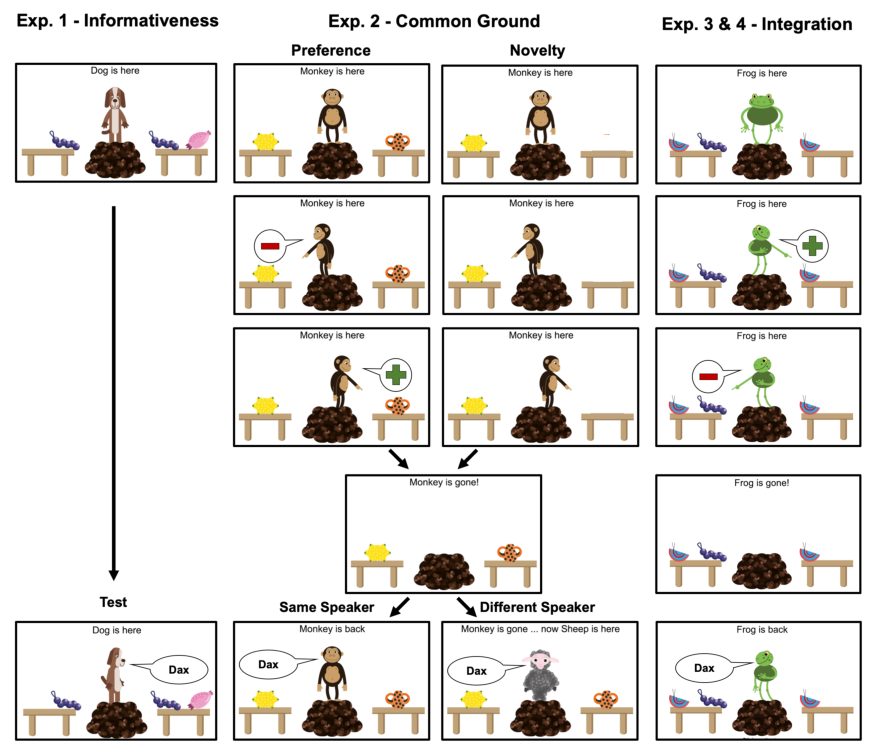
\includegraphics{figs/design-1} 

}

\caption[Schematic experimental procedure]{Schematic experimental procedure. In all conditions, at test (bottom), the speaker ambiguously requested an object using a non-word (e.g. “dax”). Participants clicked on the object they thought the speaker referred to. Informativeness (Experiment 1, left) translated to making one object less frequent in context. Common ground (Experiment 2, middle) was manipulated by making one object prefered by, or new to the speaker. Experiment 3 (right) combined manipulations. When expressing e.g. preference for an object on a table with two objects (panel 3 from top), the respective object was temporally enlarged. Condition shown here: preference - same speaker - incongruent.}\label{fig:design}
\end{figure*}
\end{CodeChunk}

\section{Experiment 1}\label{experiment-1}

\subsection{Participants, Design and
Procedure}\label{participants-design-and-procedure}

All participants were recruited from Amazon Mechanical Turk and had US
IP addresses. We planned the sample size in each experiment to be 120
data points per cell. Experiment 1 had 40 participants.Informativeness
was manipulated by making one object less frequent in context. In the
test condition, one table contained one object of type A and the other
table contained one object of type A and one of type B (see Figure 1 in
red). On each trial, the animal introduced themselves, turned towards
the table with the two objects and made a request. If listeners expect
speakers to produce informative utterances, they should select object B.
This choice follows from the counterfactual inference that if the
(informative) speaker would have wanted to request A, they would have
turned to the table that only contained A. On the other hand, since B is
only located on the table together with A, there was no alternative way
to request B in a less ambiguous way. In the control condition, both
tables contained two objects, one of which was randomly determined as
the correct one. No inference was therefore licenced based on the
animals turning. Each participant received three trials in each
condition.

\subsection{Results and Discussion}\label{results-and-discussion}

Participants selected the less frequent object above chance in the test
condition (t = 5.51, \emph{p} \textless{} .001, see Figure
\ref{fig:plotexp12}) and did so more often compared to the control
condition (genreralized linear mixed model
(GLMM\footnote{All models included random effects for subject and speaker (animal).}):\emph{\(\beta\)}
= 1.49, se = 0.5 \emph{p} = .003). This result replicates earlier work
(Frank \& Goodman, 2014).

\begin{CodeChunk}
\begin{figure}[H]

{\centering 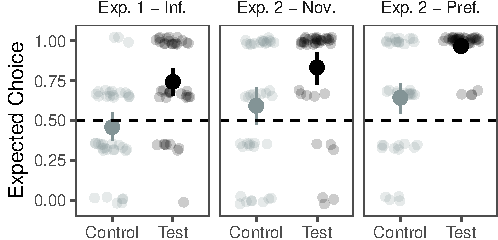
\includegraphics{figs/plotexp12-1} 

}

\caption[Results from Experiment 1 and 2.For preference and novelty, control refers to a different speaker (see Fig]{Results from Experiment 1 and 2.For preference and novelty, control refers to a different speaker (see Fig. 1). Transparent dots show data from individual particpants, solid dots represent condition means, error bars are 95 \% CIs. Dashed line indicates performance expected by chance.}\label{fig:plotexp12}
\end{figure}
\end{CodeChunk}

\section{Experiment 2}\label{experiment-2}

We manipulated common ground expectations based on two ways which have
succesfully been used in developmental studies (e.g. Akhtar et al.,
1996; Saylor et al., 2009). Speakers either expressed preference for one
object or one object was new to the speaker.

\subsection{Participants, Design and
Procedure}\label{participants-design-and-procedure-1}

There were 80 participants, 40 per manipulation. In the preference
manipulation, each table had a different object. In the beginning, the
animal appeared on the hill and introduced themselves. Next, they turned
to one of the tables and expressed either that they liked (``Oh wow, I
really like that one'') or disliked (``Oh bleh, I really don't like that
one'') the object before turning to the other side and expressing the
respective other attitude. Then, the animal disappeared. After a short
period of time, either the same or a different animal appeared and
requested an object while facing straight (see Figure 1 in blue). If
participants took into account the information they gained about the
speaker, they should select the previously preferred object if the
returning animal was the same. If a different animal returned, they
should choose randomly between objects.

In the novelty manipulation, one table was initially empty while there
was an object on the other one (see Figure \ref{fig:design}). The animal
turned to one of the sides and commented either on the presence (``Aha,
look at that'') or the absence of an object (``Hm, nothing there'').
Next, the animal quickly disappeared. The same animal re-appeared and
the sequence above was repeated. When the animal disappeared for the
second time, a second object appeared on the empty table while the
animal was away. Like in preference, we now manipulated if the same
animal or a different one would return. In case of the same animal
returning, listeners could infer the referent of the subsequent request
by considering that one object was new to the speaker and therefore more
likely to be of interest to them. No such inference was licensed when a
different animal returned because both objects were equally new to them.

\subsection{Results and Discussion}\label{results-and-discussion-1}

Participants selected the preferred object above chance when the same
animal returned (t = 29.14, \emph{p} \textless{} .001, see Figure
\ref{fig:plotexp12}) and did so more often compared to trials in which a
different animal returned (GLMM: \(\beta\) = 2.97, se = 0.7, \emph{p}
\textless{} .001). Thus, listeners inferred the referent of the
utterance by considering previous interactions with the speaker.
Interestingly, participants to some extend transferred preference from
one animal to the other and also selected the preferred object above
chance when a different animal returned (t = 2.7, \emph{p} = .01). In
sum, this study shows that adults make comparable infernces to children
(Saylor et al., 2009).

The novel object was selected above chance when the same animal returned
(t = 6.77, \emph{p} \textless{} .001) but not when a different one
appeared (t = 1.49, \emph{p} = .144, see Figure \ref{fig:plotexp12}).
Furthermore, the two conditions differed in the expected direction
(\(\beta\) = 1.7, se = 0.39, \emph{p} \textless{} .001). Thus, like
children (Akhtar et al., 1996), participants used their prior
information about the speaker to resolve ambiguity in their utterance.

\section{Experiment 3}\label{experiment-3}

\begin{CodeChunk}
\begin{figure*}[h]

{\centering 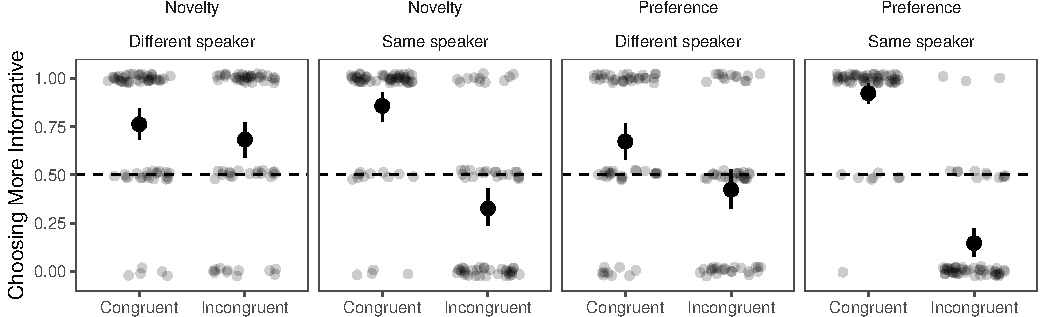
\includegraphics{figs/plotexp3-1} 

}

\caption[Results from Experiment 3]{Results from Experiment 3. Dashed line indicates performance expected by chance. Plotting conventions are the same as in Figure 2. All conditions in which CIs do not overlap with chance line are also statistically different from chance based on two-tailed Wilcoxon tests.}\label{fig:plotexp3}
\end{figure*}
\end{CodeChunk}

Experiment 1 and 2 separately measured two types of pragmatic
inferences. The first was based on the expectation that speakers produce
informative utterances. The second was based on the expectations that
speakers produce their utterances in light of the ongoing social
interaction (common ground). In Experiment 3, we combined both types of
expectations to study how listeners integrate them.

\subsection{Participants, Design and
Procedure}\label{participants-design-and-procedure-2}

A total of 121 individuals participated in the experiment. The test
situation was the same as in the test condition in Experiment 1: One
table with object of type A and the other with an object of type A and
B. Again, the animal always turned to the table with two objects and
ambiguously requested an object. In Experiment 1, the listener had no
prior information about each object. In Experiment 3, however, we
manipulated common ground expectations in the same way as in Experiment
2. For example, the animal would turn to the table with one object and
express their dis-liking of object A, then they would turn to the other
table and express their liking of object B (not using labels). Next,
after quickly disappearing, the animal would reappear, turn to the table
with two objects and make a request.

For each version of Experiment 2, there were 4 conditions in Experiment
3. If the preferred/novel object was the less frequent one (object B),
the two expectations were congruent. If the preferred/novel object was
the more frequent one (object A), expectations were incongruent. For
each type of expectation alignment, we varied if the same or a different
animal returned. Participants either completed the preference or novelty
version and received two test trials in each of the four conditions.
Before discussing the empirical results, we briefly discuss the
cognitive model we used to predict expectation integration.

\subsection{Model Predictions}\label{model-predictions}

To derive predictions, we used a probabilistic RSA model that simulates
a pragmatic listener reasoning about a cooperative speaker who is trying
to refer to an object (Frank \& Goodman, 2012). The speaker chooses how
to refer to the object by reasoning about a naive listener who does not
know the labels for the object (Frank \& Goodman, 2014). Mathematically,
the probability that the listener chooses a referent given an utterance
is defined as follows:\\
\[P_L(r_s|u)\propto P_S(u|r_s)P_S(r_s)\] Here, \(P_S(u|r_s)\) is the
likelihood that the speaker will use an utterance to refer to a specific
referent. It is defined as the surprisal of an utterance given the
referent for a naive listener, who interprets utterances in a literal
way:

\[P_S(u|r_s)\propto exp(\alpha U_S(u;s))\]

The numerical strength of the expression above depends on \(\alpha\),
which can be interpreted as an indicator of how rational the speaker is
in choosing utterances.

The term \(P_S(r_s)\) denotes the prior probability that a speaker will
refer to a given referent. This probability represents the listeners
expectations about the speaker depending on the manipulation (preference
or novelty) and the identity of the speaker (same or different speaker).

In our model, we used the results from Experiment 1 and 2 to specify
\(\alpha\) as well as \(P_S(r_s)\). The former was set to yield the
proportion measured in Experiment 1 in a model with uniform priors. The
prior probability for each object was the proportion with which this
object was chosen in Experiment
2\footnote{Proportions were measured when participants chose between two objects. However, in Experiment 3, three objects were involved. For each object we used the proportion measured in Experiment 2 as the prior probability.This approached spread out the absolute probability mass for each object but conserved the relative relation between objects.}.
Based on these parameter settings, we predicted the proportion with
which listeners will choose the less frequent object in each unique
combination of alignment and speaker identity separately for each prior
manipulation (eight conditions total, see Figure \ref{fig:plotexp3}). We
compared the fit of this pragmatic model to two alternative models using
Bayes Factors (BF). The first alternative model ignored the speaker
specific expectations (flat prior model) while the second ignored the
informativeness inference (prior only model). To capture the idea that
behavioral data is to some degree noisy, all models included a noise
parameter, which reflects that, with a certain probability, participants
respond randomly instead of in line with the intended manipulation on a
given trial. Noise parameters are estimated based on the data.

\subsection{Results and Discussion}\label{results-and-discussion-2}

\begin{CodeChunk}
\begin{figure*}[h]

{\centering 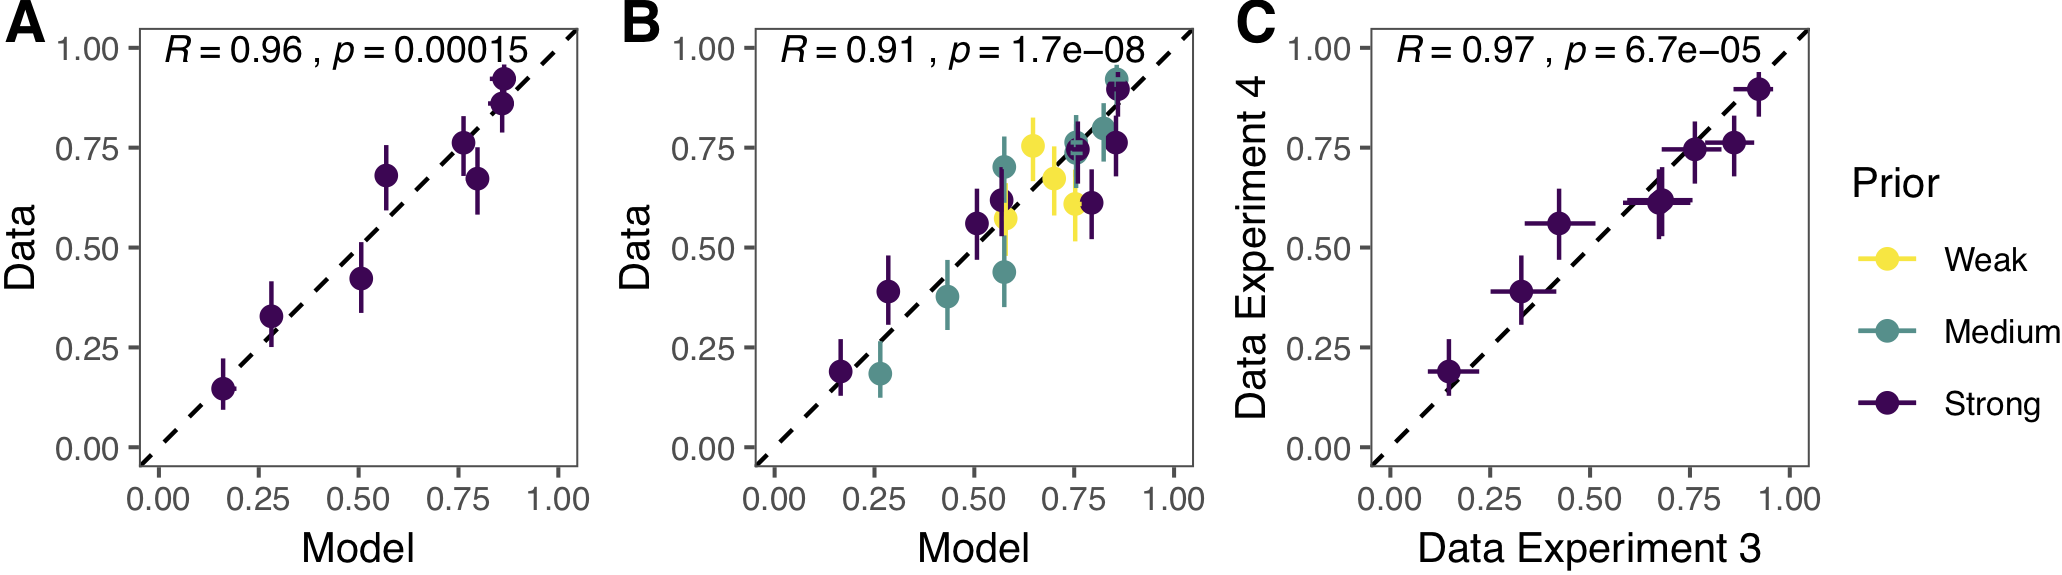
\includegraphics{figs/plotmodelcomp-1} 

}

\caption[(A) Model predictions compared to data for Experiment 3 and (B) Experiment 4]{(A) Model predictions compared to data for Experiment 3 and (B) Experiment 4. (C) Data for strong prior manipualtion in Experiment 3 and 4. Error bars = 95 \%  HDIs.}\label{fig:plotmodelcomp}
\end{figure*}
\end{CodeChunk}

Results are discussed in the form of the proportion with which listeners
chose the less frequent object. For a comparison to chance within each
unique condition see Figure \ref{fig:plotexp3}. Both alignment and
speaker identity influenced participants' responses (GLMM model term:
\texttt{alignment*speaker}; \(\beta\) = -2.92, se = 0.57, \emph{p}
\textless{} .001). Figure \ref{fig:plotmodelcomp} shows the mean
response in each unique condition compared to the model. Model
predictions and data were highly correlated (r = 0.96, \emph{p}
\textless{} .001). Model fit was better in the model taking into account
both types of expectations compared to the flat prior (BF = 2e+79) or
prior only model (BF = 1.8e+34).

Interestingly, like in Experiment 2, there was a transfer of preference
in case of a speaker change. Participants were at chance in the
preference - different speaker - incongruent condition (see Figure
\ref{fig:plotexp3}). If preference would have been specific to a
particular individual, participants should have selected the less
frequent object above chance (as they did in the corresponding condition
with the novelty manipulation).

\section{Experiment 4}\label{experiment-4}

In Experiment 4, we replicated and extended Experiment 3 by manipulating
the strength of the common ground expectations. Our main goal was to
investigate the scope of our cognitive model and we therefore limit the
description of the methods and the discussion of the results to the
aspects relevant to the comparison between model predictions and data.

\subsection{Participants, Design and
Procedure}\label{participants-design-and-procedure-3}

This experiment had 453 participants. The structure of the experiment
was the same as in Experiment 3. For each common ground expectation
(preference and novelty), we intended to have a strong, a medium and a
weak manipulation. The strength of each manipulation was determined by
the proportion with which participants chose the preferred / novel
object given the manipulation. We succeeded in this for novelty. For
preference we did not find a manipulation that yielded only a weak
preference.

The strong manipulations were identical to Experiment 3 and the results
are therefore a direct replication. For novelty, in the medium
manipulation, the animal turned to each table only once before the test.
In the weak manipulation, the animal only turned to the table with an
object before the test. In the medium manipulation for preference, the
animal only expressed liking and did so in a more subtle way (saying
only: ``Oh, wow''). Participants were assigned to one level of common
ground expectation and completed two test trials in each of the four
conditions.

Model predictions were obtained in the same way as in Experiment 3. The
likelihood term of the model was identical. For the each level of common
ground expectation, we measured the proportion with which participants
chose the preferred / novel object in a separate experiment. Due to
space limitations, we do not discuss them in any more detail here. Like
in Experiment 3, the results of these experiments were used to specify
the prior distribution in the model.

\subsection{Results and Discussion}\label{results-and-discussion-3}

As noted above, the strong prior manipulation was a direct replication
of Experiment 3. Results from the two rounds of data collection were
highly correlated (r = 0.97, \emph{p} \textless{} .001, see Figure
\ref{fig:plotmodelcomp}C). Across levels of prior manipulation, the data
from Experiment 4 were highly correlated to the corresponding model
predictions (r = 0.91, \emph{p} \textless{} .001, see Figure
\ref{fig:plotmodelcomp}B). Again, the pragmatic model provided a better
fit compared to the flat prior (BF = 4.4e+74 ) or prior only model (BF =
1.8e+84).

\section{Discussion}\label{discussion}

Language use and learning requires balancing different types of
expectations about one's interlocutor. Here we used a Bayesian cognitive
model to predict this integration process. Experiment 1 and 2 replicated
earlier studies showing that adult listeners expect speakers to produce
utterances in an informative way as well as in light of common ground.
Next, we combined the procedures from the first two experiments to study
how listeners would integrate them. We used the results from Experiment
1 and 2 to specify the model parameters that represented the two types
of expectations and make parameter-free predictions about new behavior.
Experiments 3 and 4 showed that both types of expectations influenced
listeners inferences. In general, listener behavior accurately described
by our model, suggesting that -- at least in population aggregate --
listeners trade off flexibly between speaker specific and general
pragmatic expectations.

Notably, Experiment 3 also included situations in which the two
expectations were in conflict. For example, in some trials the animal
expressed preference for object A, which was also the more frequent
object. In these situations, participants chose the preferred object as
the referent (see also Figure \ref{fig:plotexp3}). A simple explanation
for this pattern might be that common ground manipulations were simply
``stronger'' in that they produced higher rates of expected choice when
presented on their own (see Figure \ref{fig:plotexp12}). However, in
Experiment 4 we observed the same pattern in the medium manipulation for
novelty (results not discussed above, see online repository for details)
even though the manipulation alone yielded numerically weaker results
compared to the general expectation in Experiment 1. In each case, the
pattern in the data was predicted by the model This illustrates the
conditional nature of pragmatic inference: The informativeness of an
utterance critically depends on the context, including common ground. If
prior interactions already single out one object as the more likely
referent, subsequent considerations of informativeness take place in
light of this prior information and not independent of it.

In our model, we treated common ground expectations as equivalent to
more basic manipulations of contextual salience (e.g.~in Frank \&
Goodman, 2012) and did not explicitly model the social-cognitive
processes that give rise to these expectations. The interaction around
the object prior to the test event simply increased the probability that
this particular speaker will refer to the object subsequently. The same
change could be brought about if one of the objects would be made
perceptually more salient, for example by making it flash. In future
work, it would be interesting to explore ways to model common ground
expectations explicitly as well as to contrast perceptual and
interactional salience.

A logical next step will be to extend the work presented here to
children. As outlined above, pragmatic reasoning is though to play an
important role in how children learn new words. An ontogenetic study
would also show to what extent the modelling approach taken here is
suitable to address questions about development. Another fruitful future
direction would be to experimentally manipulate expectations about
speaker informativeness. For example, if a speaker repeatedly behaves in
an irrational way (e.g.~labels dogs as cats), listeners might be less
inclined to assume that utterances containing novel words are produced
in an informative way.

This work integrates different perspectives on the study of pragmatic
inference. Previous work focused either on general or speaker specific
expectations. The methodological approach taken here illustrates how
computational and experimental approaches can be used in conjunction to
explicate theories of language use and learning.

\vspace{1em}
\fbox{\parbox[b][][c]{7.3cm}{\centering Corresponding data and code are available at\ \url{https://github.com/manuelbohn/mcc}}}
\vspace{1em}

\section{Acknowledgements}\label{acknowledgements}

MB received funding from the European Union's Horizon 2020 research and
innovation programme under the Marie Sklodowska-Curie grant agreement No
749229.

\section{References}\label{references}

\setlength{\parindent}{-0.1in} \setlength{\leftskip}{0.125in} \noindent

\hypertarget{refs}{}
\hypertarget{ref-akhtar1996role}{}
Akhtar, N., Carpenter, M., \& Tomasello, M. (1996). The role of
discourse novelty in early word learning. \emph{Child Development},
\emph{67}(2), 635--645.

\hypertarget{ref-bohn2018common}{}
Bohn, M., \& Koymen, B. (2018). Common ground and development.
\emph{Child Development Perspectives}, \emph{12}(2), 104--108.

\hypertarget{ref-clark2009first}{}
Clark, E. V. (2009). \emph{First language acquisition}. Cambridge
University Press.

\hypertarget{ref-clark1996using}{}
Clark, H. H. (1996). \emph{Using language}. Cambridge University Press.

\hypertarget{ref-frank2012predicting}{}
Frank, M. C., \& Goodman, N. D. (2012). Predicting pragmatic reasoning
in language games. \emph{Science}, \emph{336}(6084), 998--998.

\hypertarget{ref-frank2014inferring}{}
Frank, M. C., \& Goodman, N. D. (2014). Inferring word meanings by
assuming that speakers are informative. \emph{Cognitive Psychology},
\emph{75}, 80--96.

\hypertarget{ref-goodman2016pragmatic}{}
Goodman, N. D., \& Frank, M. C. (2016). Pragmatic language
interpretation as probabilistic inference. \emph{Trends in Cognitive
Sciences}, \emph{20}(11), 818--829.

\hypertarget{ref-grice1991studies}{}
Grice, H. P. (1991). \emph{Studies in the way of words}. Harvard
University Press.

\hypertarget{ref-levinson2000presumptive}{}
Levinson, S. C. (2000). \emph{Presumptive meanings: The theory of
generalized conversational implicature}. MIT press.

\hypertarget{ref-saylor2009preschoolers}{}
Saylor, M. M., Sabbagh, M. A., Fortuna, A., \& Troseth, G. (2009).
Preschoolers use speakers' preferences to learn words. \emph{Cognitive
Development}, \emph{24}(2), 125--132.

\hypertarget{ref-sperber2001relevance}{}
Sperber, D., \& Wilson, D. (2001). \emph{Relevance: Communication and
cognition} (2nd ed.). Oxford; Cambridge, MA: Blackwell Publishers.

\hypertarget{ref-tomasello2009constructing}{}
Tomasello, M. (2009). \emph{Constructing a language}. Harvard university
press.

\bibliographystyle{apacite}


\end{document}
